\begin{pa} \label{PA:11.9} Consider the double integral
\begin{equation} \label{eq:11.9.COV_PA}
I = \iint_D x^2+y^2 \, dA,
\end{equation}
where $D$ is the upper half of the unit disk.
    \begin{enumerate}
    \item[(a)] Write the double integral $I$ given in Equation~(\ref{eq:11.9.COV_PA}) as an iterated integral in rectangular coordinates.

    \item[(b)] Write the double integral $I$ given in Equation~ (\ref{eq:11.9.COV_PA}) as an iterated integral in polar coordinates.


\end{enumerate}

\noindent When we write the double integral (\ref{eq:11.9.COV_PA}) as an iterated integral in polar coordinates we make a change of variables, namely
    \begin{equation}
x = r \cos(\theta)  \ \ \ \ \ \text{ and } \ \ \ \ \ y = r \sin(\theta).\label{eq:11.9.pol_to_rect}
\end{equation}
We also then have to change $dA$ to $r \, dr \, d\theta$. This process also identifies a ``polar rectangle'' $[r_1, r_2] \times [\theta_1, \theta_2]$ with the original Cartesian rectangle, under the transformation\footnote{A \emph{transformation} is another name for function:  here, the equations $x = r\cos(\theta)$ and $y = r\sin(\theta)$ define a function $T(r, \theta) = (r\cos(\theta), r\sin(\theta))$ so that $T$ is a function (transformation) from $\R^2$ to $\R^2$.  We view this transformation as mapping a version of the $x$-$y$ plane where the axes are viewed as representing $r$ and $\theta$ (the $r$-$\theta$ plane) to the familiar $x$-$y$ plane.} in Equation (\ref{eq:11.9.pol_to_rect}). The vertices of the polar rectangle are transformed into the vertices of a closed and bounded region in rectangular coordinates. 

\noindent To work with a numerical example, let's now consider the polar rectangle $P$ given by $[1, 2] \times [\frac{\pi}{6}, \frac{\pi}{4}]$, so that  $r_1 = 1$, $r_2=2$, $\theta_1 = \frac{\pi}{6}$, and $\theta_2 = \frac{\pi}{4}$. \\

    \begin{enumerate}
    \item[(c)] Use the transformation determined by the equations in~(\ref{eq:11.9.pol_to_rect}) to find the rectangular vertices that correspond to the polar vertices in the polar rectangle $P$. In other words, by substituting appropriate values of $r$ and $\theta$ into the two equations in~(\ref{eq:11.9.pol_to_rect}), find the values of the corresponding $x$ and $y$ coordinates for the vertices of the polar rectangle $P$. Label the point that corresponds to the polar vertex $(r_1, \theta_1)$ as $(x_1, y_1)$, the point corresponding to the polar vertex $(r_2, \theta_1)$ as $(x_2, y_2)$, the point corresponding to the polar vertex $(r_1, \theta_2)$ as $(x_3, y_3)$, and the point corresponding to the polar vertex $(r_2, \theta_2)$ as $(x_4, y_4)$.


    \item[(d)] Draw a picture of the figure in rectangular coordinates that has the points $(x_1,y_1)$, $(x_2,y_2)$, $(x_3, y_3)$, and $(x_4,y_4)$ as vertices. (Note carefully that because of the trigonometric functions in the transformation, this region will not look like a Cartesian rectangle.) What is the area of this region in rectangular coordinates? How does this area compare to the area of the original polar rectangle?

    \end{enumerate}
  

\end{pa}


\begin{activitySolution}
    \ba
    \item The double integral (\ref{eq:11.9.COV_PA}) can be evaluated in rectangular coordinates as the iterated integral
\[\int_{-1}^1 \int_{0}^{\sqrt{1-x^2}} x^2 + y^2 \, dy \, dx.\]


    \item By making the change of variables $x = r\cos(\theta)$ and $y = r\sin(\theta)$, and $dA = r \, dr \, d\theta$, we express the double integral (\ref{eq:11.9.COV_PA}) as the iterated integral
\[\int_0^{\pi} \int_0^1 r^2 r \, dr \, d\theta\]
in polar coordinates.

    \item Under the transformations in (\ref{eq:11.9.pol_to_rect})
\begin{itemize}
\item the vertex $(r_1, \theta_1) = \left(1, \frac{\pi}{6}\right)$ is sent to the point $(x_1, y_1) = \left(\frac{\sqrt{3}}{2}, \frac{1}{2}\right)$,
\item the vertex $(r_2, \theta_1) = \left(2, \frac{\pi}{6}\right)$ is sent to the point $(x_2, y_2) = \left(\sqrt{3}, 1 \right)$,
\item the vertex $(r_1, \theta_2) = \left(1, \frac{\pi}{4}\right)$ is sent to the point $(x_3, y_3) = \left(\frac{\sqrt{2}}{2}, \frac{\sqrt{2}}{2}\right)$,
\item the vertex $(r_2, \theta_2) = \left(2, \frac{\pi}{4}\right)$ is sent to the point $(x_4, y_4) = \left(\sqrt{2}, \sqrt{2}\right)$.
\end{itemize}

    \item If we lived in polar coordinates, the polar rectangle $P$ would look to us as shown below at left. The image $P'$ of the polar rectangle $P$ under the transformations in (\ref{eq:11.9.pol_to_rect}) is shown below at right.
%\begin{figure}[h]
\begin{center}
%\begin{minipage}{2.5in}
%\begin{center}
\resizebox{!}{2.4in}{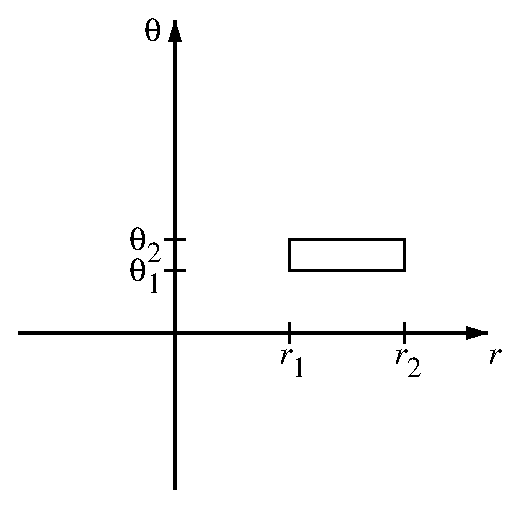
\includegraphics{figures/fig_11_9_Polar_COV_1}}
%\end{center}
%\caption{Rectangle $P$ in the polar world.}
%\label{F:11.9.Change_vars1_a}
%\end{minipage}
\hspace{0.25in}
%\begin{minipage}{2.5in}
%\begin{center}
\resizebox{!}{2.4in}{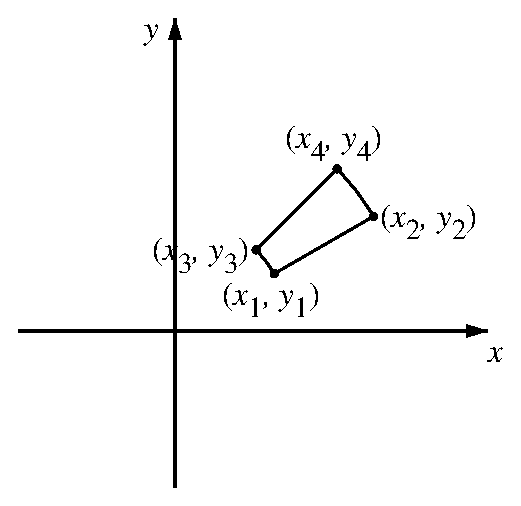
\includegraphics{figures/fig_11_9_Polar_COV_2}}
%\end{center}
%\caption{Image $P'$ in the Cartesian world.}
%\label{F:11.9.Change_vars1_b}
%\end{minipage}
\end{center}
%\end{figure}
We have seen that the area of the transformed rectangle $P'$ is given by $\frac{r_2+r_1}{2} \Delta r \Delta \theta$, and as $\Delta r$ and $\Delta \theta$ go to 0 this area becomes the area element $dA = r \, dr \, d\theta$. This is the general idea of a change of variables in multiple integrals.

	\ea
	
\end{activitySolution}

 \afterpa 